Um die Molwärme berechnen zu können, müssen zunächst die spezifischen
Wärmekapazitäten der einzelnen Proben und die des Kalorimeters
experimentell bestimmt werden.
Die Molwärme lässt sich dann ohne weitere experimentelle Durchführungen
berechnen.
\subsection{Bestimmung der spezifischen Wärmekapazität des Kalorimeters}
% Zuerst wird die Masse $m_\su{k}$ der Probe mit einer Schnellwaage ermittelt.
% Danach wird diese in einem Wasserbad auf eine Temperatur $T_\su{k}$ von
% mindestens $60\,\si{\celsius}$ erhitzt.
\begin{figure}
  \centering
  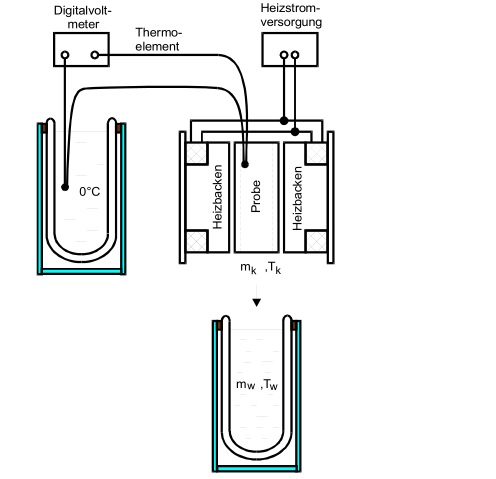
\includegraphics[width=0.8\textwidth]{bilder/aufbau.jpg}
  \caption{Schemtischer Aufbau\,\cite{201}}
  \label{aufbau}
\end{figure}
Um die spezifische Wärmekapazität des Kalorimeters zu bestimmen, wird dieses
mit einer bestimmten Menge Wasser gefüllt. Die Temperatur der Wände $T_\su{w}$
wird gemessen, wenn sich die Temperaturen des Wassers an die Kalorimeter-Wand
angleichen. Als nächstes wird die verbleibende Wassermenge im Kalorimeter
bestimmt, indem etwa die Hälfte des Wassers aus dem Kalorimeter entfernt und
gewogen wird. Zusätzlich wird die Wassermenge gewogen, die anschließend erhitzt wird,
da es nicht möglich ist, die gesamte Wassermenge in zwei exakt gleich große
Mengen aufzuteilen.
Das Wasser wird auf einer Heizplatte erhitzt bis es siedet und dann
wieder zurück in das Kalorimeter gegeben. Die Mischtemperatur wird gemessen, sobald
diese sich einstellt. Die Messung wird dreimal durchgeführt um systematische
Fehler zu minimieren. Ein schematischer Aufbau ist in Abbildung \ref{aufbau}
zu sehen.
\subsection{Bestimmung der spezifischen Wärmekapazität der Proben}
Zunächst wird die Probenmasse mittels einer Schnellwaage bestimmt. Dann wird die
Probe in siedendem Wasser erwärmt, bis sie eine Temperatur von $373.15\Kel$
erreicht. Gleichzeitig wird eine bestimmte Menge Wasser in das Kalorimeter
gefüllt und die Temperatur gemessen. Dabei ist zu beachten, dass dies dieselbe
Menge Wasser ist, welche auch bei der Kalorimetermessung verwendet wird.
Die Probe wird in das Kalorimeter getaucht,
sobald dieses die Temperatur des Wassers annimmt. Die Mischtemperatur $T_\su{m}$
wird gemessen, sobald sich ein thermisches Gleichgewicht eingestellt.
Gemessen werden Proben von Blei, Graphit und Aluminium. Die Messung für Blei
und Aluminium wird dreimal durchgeführt, die für Graphit jedoch nur einmal.
